\documentclass[11pt, a4paper, oneside]{article} % article scrartcl
\usepackage[utf8x]{inputenc}		% Umlaute können genutzt werden ohne \" davor zu stellen
\usepackage{ucs}					% contains support for using UTF-8 as input encoding
\usepackage{amsmath}				% besser Mathe-Ausgabe
\usepackage{amsfonts}				% Mathe-Schrift
\usepackage{amssymb}				% Mathe-Symbole
\usepackage[ngerman]{babel}			% für deutsche Sprache. Übersetzungen (z.Bsp. Zusammenfassung <-- Abstract) und Silbentrennung 
\usepackage{fancyhdr}				% für Kopf- und Fußzeilen
\usepackage{graphicx}				% für Bilder
\usepackage{graphics}				% für Bilder
\usepackage{url}					% für anklickbare URLs
\usepackage{parskip}				% kein Einrücken sondern Leerzeilen zwischen Abschnitten
\usepackage{color}					% Farben
\usepackage{units}   				% Einheiten, \unit[23]{m}
\usepackage{hyperref}				% Referenzen
\usepackage{todonotes}				% Todonotes im Text 
\usepackage{listings}				% sourcecode
\usepackage{grffile}				% graphic filename extensions
\usepackage{lscape}					% landscape
\usepackage{pdflscape}				% landscape, if using PDFLaTeX
\usepackage{geometry}

\definecolor{dkgreen}{rgb}{0,0.6,0}
\definecolor{gray}{rgb}{0.5,0.5,0.5}
\definecolor{mauve}{rgb}{0.58,0,0.82}
 
\lstset{ %
  language=Java,               		% the language of the code
  basicstyle=\footnotesize,         % the size of the fonts that are used for the code
  numbers=left,                   	% where to put the line-numbers
  numberstyle=\footnotesize,        % the size of the fonts that are used for the line-numbers
  stepnumber=1,                  	% the step between two line-numbers. If it's 1, each line 
                                  	% will be numbered
  numbersep=6pt,                  	% how far the line-numbers are from the code
  backgroundcolor=\color{white},    % choose the background color. You must add \usepackage{color}
  showspaces=false,               	% show spaces adding particular underscores
  showstringspaces=false,         	% underline spaces within strings
  showtabs=false,                 	% show tabs within strings adding particular underscores
  frame=single,                   	% adds a frame around the code
  tabsize=2,                      	% sets default tabsize to 2 spaces
  captionpos=t,                   	% sets the caption-position to bottom
  breaklines=true,                	% sets automatic line breaking
  breakatwhitespace=false,        	% sets if automatic breaks should only happen at whitespace
  title=\lstname,                   % show the filename of files included with \lstinputlisting;
                                  	% also try caption instead of title
  numberstyle=\tiny\color{gray},    % line number style
  keywordstyle=\color{blue},        % keyword style
  commentstyle=\color{dkgreen},     % comment style
  stringstyle=\color{mauve},        % string literal style
  escapeinside={(*@}{@*)},          % if you want to add a comment within your code    %   \%*}{*)
  morekeywords={*,...},              % if you want to add more keywords to the set    
  literate={ö}{{\"o}}1
           {ä}{{\"a}}1
           {ü}{{\"u}}1
           {ß}{{\ss}}1
}

% Ränder
\geometry{paper=a4paper,left=30mm,right=30mm,top=25mm, bottom=25mm}

\author{Martin Junghanns \\  \url{martin.junghanns@studserv.uni-leipzig.de} \and 
		Sascha Ludwig \\ \url{s.ludwig@studserv.uni-leipzig.de} \and 
		Robert Schulze \\ \url{robert.schulze@studserv.uni-leipzig.de} }
\date{\today}
\title{ Performanz Evaluation von Graphdatenbanksystemen versus MySQL am Beispiel von Kookkurrenzgraphen }

% Standardpfad fuer Grafiken
\graphicspath{
 {./pics/}
}


\begin{document}

% bei Aufzählungen einen Strich an Stelle eines Punktes verwenden
\renewcommand{\labelitemi}{-}

% Titel mit Autoren
\maketitle

% Abstract
\begin{abstract}
	Dieser Bericht ist die Zusammenfassung der Praktikumsergebnisse im Rahmen des Moduls \dq Fortgeschrittene Methoden des Information Retrieval\dq~im WS 2010/11 der Universität Leipzig. Inhalt des Praktikums war die Evaluation verschiedener Graphdatenbanken und die Gegenüberstellung von relationalen Datenbanken. Als Vertreter der Graphdatenbanken wurden Neo4j, DEX und OrientDB näher betrachtet, MySQL wurde als relationale Datenbank in den Vergleich einbezogen.\\
Konkrete Ziele des Praktikums waren das Kennenlernen der verschiedenen Graphdatenbanken, der zu Grunde liegenden Datenmodelle und deren Abfragetechniken. Für den experimentellen Vergleich sollten verschiedene Kookkurrenzgraphen des Wortschatz Leipzig Projektes in die jeweilige Datenbanken importiert und mit den individuell angebotenen Möglichkeiten abgefragt werden. Dabei wurden ausgewählte SQL-Anfragen in API-Anfragen, aber auch in deklarative Anfragesprachen des jeweiligen Herstellers umformuliert und hinsichtlich ihrer Ausführungszeit verglichen.\\
Um die gemessenen Ausführungszeiten besser vergleichen zu können wurden die Messergebnisse mittels genuplot\footnote{\url{http://http://www.gnuplot.info/}} visualisiert.
\end{abstract}

\section{Projektbeschreibung}
Als Ergebnis des Praktikums ergaben sich zum Einen konkrete und vergleichbare Messergebnisse der einzelnen Datenbanken. Zum Anderen ist ein minimales, einfach konfigurierbares und auf den Anwendungsfall des Vergleichs von Datenbanken angepasstes Benchmark-Framework entstanden. Das Framework unterstützte uns beim Aggregieren der Messergebnisse einzelner Datenbanken und erleichterte wiederkehrende Aufgaben. 
	
\subsection{Softwarearchitektur}
Das Framework besteht aus sechs Komponenten, durch deren Ableitung und Kombination sich ein einzelner Benchmarkvorgang durchführen lässt. Die einzelnen Komponenten werden im Folgenden kurz vorgestellt. 

\subsubsection{Konnektoren}
Ein Konnektor (Connector) dient den einzelnen Benchmarks oder Importierern zur Verwaltung der  Verbindung zu einer konkreten Datenbank. Die Verwaltung umfasst dabei den Verbindungsaufbau unter Angabe verschiedener Parameter, wie bspw. Hostnamen, Ports und Nutzerinformationen. Darüber hinaus stellen die Konnektoren auch den korrekten Abbau einer Verbindung sicher. Für jede Datenbank muss nur ein Konnektor implementiert werden.

\subsubsection{Importierer}
Ein Importierer (Importer) dient dem Laden einer Datenbasis in eine konkrete Datenbank. Im Rahmen des Praktikums wurde die Datenbasis aus einer MySQL Datenbank geladen. Eine Erweiterung des Frameworks zur Unterstützung verschiedener Datenquellen wie bspw. CSV-Dateien ist jedoch ebenfalls möglich. Für den möglichen Fall, dass Benchmarks nicht auf einer existierenden Datenbasis operieren, ist die Implementierung eines Importierers nicht notwendig. Durch den Importierer lässt sich eine Datenbank auch in den Urzustand zurücksetzen wodurch alle zuvor importierten Daten entfernt werden.

\subsubsection{Benchmark}
Innerhalb eines Benchmarks wird durch das Implementieren einer abstrakten Run Methode die eigentliche Ausführungslogik definiert. Vor- und Nachbedingungen werden in Setup und TearDown Methoden festgelegt. Die Sicherstellung dieser Bedingungen spiegelt sich somit nicht in der Ausführungszeit des Benchmarks wieder. Die Methoden werden zum Beispiel zum Parsen eines SQL- oder Cypher-Statements verwendet oder zur Auswahl des nächsten Startknotens.

\subsubsection{Benchmark-Suite}
Benchmarks werden mittels Benchmark-Suiten ausgeführt. Dabei besteht die Möglichkeit, mehrere Benchmarks mit dem Ziel zusammenzufassen, diese in einer definierten Abfolge auszuführen. Durch eine Main-Methode bietet die Benchmark-Suite einen Einstiegspunkt in die Ausführung der Benchmarks.\\
Neben den Methoden zur Ausführung von Benchmarks und der damit verbundenen Zeitmessung bieten Benchmark-Suiten die Möglichkeit, Aggregation und Persistierung von Messergebnissen durchzuführen. Diese Methoden können verwendet, oder in einer konkreten Implementierung erweitert werden.

\subsubsection{Konfigurationsdateien}
Bezüglich geeigneter Parameter ist die Konfiguration der einzelnen Datenbanken oder des Frameworks selbst über sogenannte properties-Dateien möglich (siehe dazu den Abschnitt \ref{subsubsec:benchmarks_conf}).

\subsection{Bedienungsanleitung}
\label{subsec:bedienungsanleitung}

\subsubsection{Voraussetzungen}
Um das Benchmark-Framework und die von uns implementierten Beispielabfragen ausführen zu können, ist die Installation der Java Runtime Environment 1.6\footnote{\url{http://www.java.com/en/download/manual.jsp}} und Apache Maven 2\footnote{\url{http://maven.apache.org/docs/2.2.1/release-notes.html}} notwendig. Alle weiteren genutzten Bibliotheken, wie bspw. jene der verwendeten Datenbanken, werden durch die Ausführung des entsprechenden Maven-Kommandos heruntergeladen und installiert.

Das Framework inklusive aller Benchmarks ist als Git-Versionsarchiv bei github\footnote{\url{https://github.com/s1ck/IR15}} öffentlich verfügbar. Das Versionsarchiv lässt sich als gepacktes Zip-Archiv herunterladen\footnote{\url{https://github.com/s1ck/IR15/zipball/master}}. Alternativ kann das Versionsarchiv auch mittels \texttt{git clone \url{git://github.com/s1ck/IR15.git}} ausgecheckt werden. Für einen Überblick bzgl. der Benutzung von Git als Versionsverwaltungssystem empfehlen wir das Git User´s Manual 
\footnote{\url{http://schacon.github.com/git/user-manual.html}} oder die Gitcasts\footnote{\url{http://gitcasts.com/}}.

Nachdem das Zip-Archiv entpackt wurde, werden mit Hilfe des Maven-Kommando \texttt{mvn clean install} alle Abhängigkeiten zu Bibliotheken, die durch das Framework verwendet werden, aufgelöst und dies entsprechenden Bibliotheken installiert.

\subsubsection{Benchmarks konfigurieren}
\label{subsubsec:benchmarks_conf}
Wie bereits erwähnt, lässt sich das Framework mittels properties-Dateien konfigurieren. Listing \ref{lst:inst_conf} zeigt die Konfiguration am Beispiel DEX. Dem Versionsarchiv liegen entsprechende Beispielkonfigurationen bei, die entsprechend umbenannt und angepasst werden müssen. 

\lstinputlisting
    [caption={Konfigurations der DEX-Benchmarksuite}
       \label{lst:inst_conf},language=bash]
 {../../src/main/resources/dex.properties.example}

\subsubsection{Benchmarks ausführen}
Sind alle Voraussetzungen erfüllt, lassen sich die einzelnen Benchmark-Suiten durch das Maven-Kommando \texttt{mvn exec:java} ausführen.

\begin{lstlisting}[caption={Ausführen der einzelnen Benchmarksuites},label={lst:inst_run}]
// DEX
mvn exec:java -Dexec.mainClass="de.uni.leipzig.IR15.Benchmark.suites.DEXBenchmarkSuite"

// OrientDB
mvn exec:java -Dexec.mainClass="de.uni.leipzig.IR15.Benchmark.suites.OrientBenchmarkSuite"

// Neo4j
mvn exec:java -Dexec.mainClass="de.uni.leipzig.IR15.Benchmark.suites.Neo4JBenchmarkSuite"

// MySQL
mvn exec:java -Dexec.mainClass="de.uni.leipzig.IR15.Benchmark.suites.MySQLBenchmarkSuite"
\end{lstlisting}

\subsubsection{zusätzliche Benchmarks}
Das Framework lässt sich sehr leicht um zusätzliche Benchmarks für bereits existierende Datenbanken erweitern. Dazu muss eine der Klassen \texttt{DEXBenchmark}, \texttt{MySQLBenchmark}, \texttt{Neo4jBenchmark} oder \texttt{OrientDBBenchmark} abgeleitet und die entsprechenden Methoden implementiert werden. Dabei sollte man sich an den vorhandenen Benchmarks orientieren. Als nächstes muss der zusätzliche Benchmark in die entsprechende Benchmarksuite (\texttt{DEXBenchmarkSuite}, \linebreak\texttt{MySQLBenchmarkSuite}, \texttt{Neo4JBenchmarkSuite} oder \texttt{OrientBenchmarkSuite}) aufgenommen werden, damit dieser auch ausgeführt wird. Als letztes empfiehlt sich, ein zusätzliches property in der zugehörigen properties-Datei einzuführen, damit auch das ergänzte Benchmark wie alle anderen ein- bzw. ausgeschaltet werden kann.

\subsubsection{zusätzliche Datenbank}
Um das Framework um Benchmarks für eine zusätzliche Datenbank zu erweitern sind mehrere Schritte notwendig. Diese sollen im Folgenden nur genannt und nicht im Detail beschrieben werden. Der vorhandene Quellcode ist umfangreich dokumentiert und kommentiert, so dass man sich an den Implementierungen für die bereits genutzten Datenbanken orientieren kann. 

Es empfiehlt sich dabei stets alle datenbank-, system- oder benchmarkabhängigen Einstellungen in eine properties-Datei auszulagern um diese besser anpassen zu können, ohne dass der Quellcode vor der Ausführung neu kompiliert werden muss.

Im ersten Schritt muss für eine neue zusätzliche Datenbank ein Konnektor implementiert werden. Unsere Konventionen geben vor, dass dieser mindestens die Methoden \texttt{getConnection} zum Aufbau, \texttt{destroyConnection} zum Schließen der Verbindung zur Datenbank und \texttt{reset }zum Zurücksetzen der Datenbank implementiert.

Damit die zusätzliche Datenbank mit einer Datenbasis gefüllt werden kann, muss ein Importierer implementiert werden. Dieser leitet sich von der Klasse \texttt{Importer} ab und implementiert mindestens die Methoden \texttt{setUp}, \texttt{tearDown} und \texttt{importData}.

Einzelne Benchmarks werden, wie schon erwähnt, in einer Benchmark-Suite zusammengefasst und durch diese ausgeführt. Eine Benchmark-Suite wird von der Klasse \texttt{AbstractBenchmarkSuite} abgeleitet und ist das eigentliche ausführbare Java-Programm, in dessen \texttt{main}-Methode, die einzelnen Benchmarks initialisiert und ausgeführt werden.

Angenommen, das Framework soll um die Datenbank MongoDB\footnote{\url{http://www.mongodb.org/}} erweitert werden, dann sollten mindestens die Klassen \texttt{MongoDBConnector}, \texttt{MongoDBImporter}, \texttt{MongoDBBenchmarkSuite} und \texttt{MongoDBBenchmark} implementiert werden. Abbildung \ref{fig:class_diagramm_neo4j} zeigt das Klassendiagramm am Beispiel der Implementierungen für Neo4j, dort sind die Zusammenhänge der einzelnen Klassen zu erkennen. Die Klassendiagramme der Implementierungen von DEX und OrientDB sind äquivalent.

\subsection{Einschränkungen}

Vorhandene Einschränkungen Datenbank-spezifischer Natur sind im jeweiligen Abschnitt dokumentiert.

An dieser Stelle sei darauf hingewiesen, dass im Rahmen des Praktikums keine überdurchschnittliche Expertise bezüglich der verwendeten Datenbanken ausgebildet werden konnte und somit die Aussagekraft der Messergebnisse unter folgenden Bedingungen zu betrachten sind: Es ist durchaus möglich, dass weitere Optimierungen der Datenbankoperationen im Rahmen der Benchmarks möglich sind. Dabei kann es sein, dass eine Optimierung nur hinsichtlich bestimmter Operationen von Vorteil ist und sich bei anderen Operationen nachteilig auswirken kann.

\subsection{Erweiterungsmöglichkeiten}

Bezüglich der Erweiterungsmöglichkeiten muss wie folgt differenziert werden: Zum Einen ist es möglich, die Benchmarks selbst zu erweitern (siehe Bedienungsanleitung im Absatz \ref{subsec:bedienungsanleitung}), zum Anderen bietet das Framework an sich Potenzial für Erweiterungen. Zwei mögliche Erweiterungen des Frameworks werden nachfolgend beschrieben.

\subsubsection*{Vereinfachte Konfiguration der Benchmark-Suiten}
Es ist vorstellbar, dass die Erstellung einer Benchmark-Suite, also das Zusammenführen einzelner Benchmarks zu einer geordneten Folge, nicht zwingend in Programmierleistung in einer Java-Klasse geschehen muss. Denkbar wäre, dass man dies lediglich in einer properties-Datei konfiguriert. Dies vereinfacht das Anpassen einer Benchmark-Suite und ist auch für Personen ohne Programmierkenntnisse möglich.

\subsubsection*{Visualisierung von Messergebnissen durch das Framework}
Momentan geschieht die Auswertung der Messergebnisse noch außerhalb des Frameworks. Hierfür existieren zusätzliche Skripte, welche die Messergebnisse aggregieren, aufbereiten und mittels R oder gnuplot visuell zugänglich ausgibt. Dieses Aggregieren und Aufbereiten der Daten und das Ansprechen von gnuplot ist auch mittels Java möglich und könnte in das Framework integriert werden.

% der wahre Inhalt
\section{Neo4j}

Neo4j\footnote{\url{http://www.neo4j.org}} ist eine eingebettete, persistente, transaktionale Graphdatenbank. Sie wird seit 2005 von der Firma Neo Technology, Inc. entwickelt, Version 1.0 erschien Anfang 2010. Die Datenbank wurde vollständig in Java geschrieben und steht quelloffen zur Verfügung.\footnote{\url{https://github.com/neo4j/community}}

\subsection{Anbindung}

Neo4j kann in zwei verschiedenen Szenarien betrieben werden: Die eingebettete Version wird direkt in eine Java Applikation integriert und bietet den performantesten Zugriff auf die Datenbank. Darüber hinaus implementiert Neo4j eine REST Schnittstelle, mit welcher auf die Datenbank via HTTP Requests zugegriffen werden kann. Die Anbindung erfolgt über verschiedene Clients, welche den Zugang aus unterschiedlichen Plattformen und Sprachen heraus ermöglichen.\\
Für die Leistungsmessung wurde die eingebettete Variante der Datenbank genutzt. Sie bietet neben dem Geschwindigkeitsvorteil auch das volle Spektrum an Zugriffsmöglichkeiten an.

\subsection{Anfragemöglichkeiten}

Neo4j bietet verschiedene Möglichkeiten an, den gespeicherten Graphen zu traversieren bzw. abzufragen. Neben der nativen Java-API und der ebenfalls in Java entwickelten Traversal API steht seit Version 1.5 mit Cypher eine deklarative Abfragesprache zur Verfügung. Die drei genannten Abfragemöglichkeiten werden im Folgenden kurz vorgestellt und anhand kurzer Beispiele erläutert.

\subsubsection{Native API}

\begin{lstlisting}[caption={Erstellen, Öffnen und Schließen einer Datenbank},label={lst:neo_create}]
// benoetigte imports
import org.neo4j.graphdb.GraphDatabaseService;
import org.neo4j.kernel.EmbeddedGraphDatabase;

// GraphDB-Objekt
GraphDatabaseService neo4j;
// Pfad zu dem Ordner, in dem die DB gespeichert werden soll
String location = "<PATH_TO_FOLDER>";
// oeffne oder erzeuge eine Datenbank
neo4j = new EmbeddedGraphDatabase(location);(*@\label{Neocreate}@*)
// ... Anweisungen ...
// Datenbank schliessen
neo4j.shutdown();(*@\label{Neoclose}@*)
\end{lstlisting}

Listing \ref{lst:neo_create} zeigt die nötigen Schritte um eine bestehende Datenbank zu öffnen, bzw. eine neue Datenbank zu erzeugen. In Zeile \ref{Neocreate} wird eine Instanz einer eingebetteten Datenbank erzeugt und gleichzeitig der Zugriff ermöglicht. Alternativ ist hier die Verbindung zu einem Neo4j Server über die angebotene REST Schnittstelle möglich. Diese Variante wurde im Rahmen des Praktikums nicht verwendet, weshalb die Verwendung nicht weiter beschrieben wird. Zum Schließen der Datenbank erfolgt ein Aufruf der \textit{shutdown} Methode (Zeile \ref{Neoclose}).
\par
Das Einfügen von Knoten (engl. \textit{nodes}) und Kanten (engl. \textit{relationships}) erfolgt über die Instanz einer Graphdatenbank. Schreiboperationen werden in Transaktionen gekapselt, damit im Fehlerfall Änderungen verworfen werden können und die Erkennung von Deadlocks durch die Datenbank ermöglicht wird. Listing \ref{lst:neo_add} zeigt hierfür ein Beispiel.

\begin{lstlisting}[caption={Einfügen von Knoten und Kanten},label={lst:neo_add}]
// Starten einer Transaktion
Transaction tx = neo4j.beginTx();
try {
	// Anlegen eines Knotens
	Node source = neo4j.createNode();(*@\label{Neoadd_createSource}@*)
	// Properties am Knoten hinzufügen
	source.setProperty("w_id", 23);(*@\label{Neoadd_addProp}@*)
	source.setProperty("word", "neo4j");
	
	// Anlegen eines weiteren Knotens	
	Node target = neo4j.createNode();
	// Properties am Knoten hinzufügen
	source.setProperty("w_id", 42);
	source.setProperty("word", "graphdb");
	
	// Anlegen einer Kante zwischen den beiden Knoten
	Relationship edge = source.createRelationshipTo(target, RelTypes.CO_N); (*@\label{Neoadd_addRel}@*)
	// Properties an der Kante hinzufügen
	edge.setProperty("freq", 7);(*@\label{Neoadd_addRelProp}@*)
	edge.setProperty("sig", 13.37);

	// Transaktion abschließen
	tx.success();
} finally {
	tx.finish();
}
\end{lstlisting}

In Zeile \ref{Neoadd_createSource} wird ein neuer Knoten erzeugt, diesem werden in den folgenden Zeilen zwei Eigenschaften (engl. \textit{properties}) zugewiesen. Nach dem Anlegen eines zweiten Knotens, werden beide Knoten in Zeile \ref{Neoadd_addRel} durch eine Kante verbunden. Der Kantentyp muss zuvor definiert werden (Listing \ref{lst:neo_relationship}). Kanten können analog zu Knoten mit Properties versehen werden.

\begin{lstlisting}[caption={Anlegen von Kantentypen},label={lst:neo_relationship}]
import org.neo4j.graphdb.RelationshipType;

public enum RelTypes implements RelationshipType {
	CO_S, // Satz-Kookkurrenz
	CO_N // Nachbarschafts-Kookkurrenz
}
\end{lstlisting}

Die Abfrage des Graphen mittels nativer API ist in Listing \ref{lst:neo_abfrage} dargestellt. Im Beispiel werden alle Satzkookkurrenzen eines Wortes (source) abgefragt. Dazu werden die entsprechenden Kanten geladen und anschließend die hinterlegten Properties abgefragt. Jede Kante beinhaltet einen Verweis auf ihren Start- und Zielknoten. In Zeile \ref{NeoNative_nodeprop} wird zunächst der Zielknoten geladen und anschließend dessen Eigenschaft \textit{w\_id}. In den darauffolgenden Zeilen werden die Eigenschaften der Satzkookkurrenz geladen.

\begin{lstlisting}[caption={Verwendung der nativen API},label={lst:neo_abfrage}]
for (Relationship e : startNode.getRelationships(RelTypes.CO_S, Direction.OUTGOING)) {
	e.getEndNode().getEndNode().getProperty("w2_id"); // w2_id (*@\label{NeoNative_nodeprop}@*)
	e.getEndNode().getProperty("sig"); // significance
	e.getEndNode().getProperty("freq"); // frequency
}
startNode.getProperty("w_id"); // w1_id 
\end{lstlisting}
 

\subsubsection{Traversal API}

Die Traversal API verwendet intern die native API, erlaubt jedoch die Formulierung komplexer, algorithmischer Graphtraversals. In Listing \ref{lst:neo_traversal} sollen alle Satzkookkurrenzen der Nachbarn eines Wortes ausgegeben werden. Über eine Traversal Description wird dabei das Traversieren des Graphen beschrieben. Dafür ist es zunächst erforderlich zwischen Breiten- und Tiefensuche zu wählen (Zeile \ref{NeoTraversal_type}). Im Anschluss wird in Zeile \ref{NeoTraversal_edges} der relevante Kantentyp und die Richtung der Kante definiert. Der ab Zeile \ref{NeoTraversal_eval} beschriebene Pfad Evaluator wertet bei jedem Hop den aktuell berechneten Pfad aus. Im Beispiel ist lediglich die Länge des Pfades entscheidend: Da nur die Nachbarn der Nachbarn von Interesse sind, wird die maximale Pfadlänge auf Zwei festgelegt. Ist die entsprechende Pfadlänge erreicht wird der aktuelle Knoten in die Ergebnismenge eingebunden und das Traversieren dieses Pfades abgebrochen, andernfalls wird der aktuelle Knoten aus dem Ergebnis ausgeschlossen, die Suche jedoch ausgehend vom aktuellen Knoten fortgesetzt. Letzteres ist notwendig, wenn alle Knoten mit einem definierten Abstand vom Startknoten gefunden werden sollen, Zwischenknoten für das Ergebnis jedoch nicht relevant sind. Zyklen werden standardmäßig vermieden, da Knoten nur einmal besucht werden können. Dies kann jedoch explizit deaktiviert werden.\\
In Zeile \ref{NeoTraversal_run} wird der Traversal mit dem Startknoten initialisiert und gestartet, das Ergebnis ist eine Menge von Pfaden. Im Beispiel ist der Endknoten eines Pfades und dessen Eigenschaft \textit{w\_id} von Interesse.

\begin{lstlisting}[caption={Verwendung der Traversal API},label={lst:neo_traversal}]
TraversalDescription td = Traversal
	.description()
	.breadthFirst() (*@\label{NeoTraversal_type}@*)
	.relationships(RelTypes.CO_S, Direction.OUTGOING) (*@\label{NeoTraversal_edges}@*)
	.evaluator(new Evaluator() { (*@\label{NeoTraversal_eval}@*)
		@Override
		public Evaluation evaluate(Path path) {
			if (path.length() == 2) {
				return Evaluation.INCLUDE_AND_PRUNE;
			} else {
				return Evaluation.EXCLUDE_AND_CONTINUE;
			}
		}
	});

for (Path p : td.traverse(startNode)) { (*@\label{NeoTraversal_run}@*)
	p.endNode().getProperty("w_id"); // w2_id
}
\end{lstlisting}

\subsubsection{Cypher}

Eine dritte Möglichkeit, Anfragen an die Graphdatenbank zu stellen, bietet die deklarative Sprache \textit{Cypher}. Sollen beispielsweise alle Nachbarn eines Knotens mit der ID 3  abgefragt werden, die über eine ausgehende Kante mit diesem Knoten verbunden sind, bietet sich folgende Query an:
\begin{lstlisting}
START n=node(3) MATCH (n)-->(x) RETURN x
\end{lstlisting}
Eine Einschränkung auf einen bestimmten Kantentyp ist ebenfalls möglich:
\begin{lstlisting}
START n=node(3) MATCH (n)-[:CO_N]->(x) RETURN x
\end{lstlisting}
Folgendes Beispiel gibt die Signifikanz aller Satzkookkurrenzen zurück, welche auf die Nachbarschaftskookkurrenzen eines Knotens verweisen:
\begin{lstlisting}
START n=node(3) MATCH (n)-[:CO_N]->()<-[r:CO_S] RETURN r.sig
\end{lstlisting}
Das folgende Listing beinhaltet eine Einschränkung durch das Prädikat $r.sig > 3$, eine Sortierung der Ergebnismenge in natürlicher Ordnung und das Einschränken auf das erste Ergebnis.
\begin{lstlisting}
START n=node(3) 
MATCH (n)-[:CO_N]->()<-[r:CO_S] 
WHERE r.sig > 3.0 
RETURN r.sig
ORDER BY r.sig
LIMIT 1
\end{lstlisting}

Die Verwendung von Cypher inerhalb von Java ist in Listing \ref{lst:neo_cypher} dargestellt.

\begin{lstlisting}[caption={Verwendung von Cypher in Java},label={lst:neo_cypher}]
// Erzeugen der Engine auf Basis einer Neo4j Instanz
ExecutionEngine engine = new ExecutionEngine(neo4j);
// Definition der Query
String cypherQuery = "START n=node(3) MATCH (n)-[:CO_N]->(x) RETURN x";
// Ausführen der Query
engine.execute(cypherQuery);
\end{lstlisting}

\subsection{Einschränkungen}

Wie im vorhergehenden Abschnitt gezeigt, ist Cypher eine einfache Möglichkeit, Abfragen auf Graphen zu formulieren. Da es sich bei der Sprache jedoch um ein noch junges Feature in Neo4j handelt, wird der Schwerpunkt momentan noch auf korrekte Funktionalität und weniger auf optimierte Ausführung gelegt. Dies führte dazu, dass bei umfangreichen Graphen die Performance im Vergleich zur nativen API deutlich geringer war und es darüber hinaus oft zu Speicherüberläufen kam. Letzteres trat auch bei der Verwendung der Traverser API auf. Wie bereits beschrieben, werden Knoten standardmäßig nur einmal besucht. Für verschiedene Graphen ist das Erkennen von Zyklen jedoch entscheidend, weswegen das mehrmalige Besuchen von Knoten erlaubt werden muss. In diesem Fall kam es häufig zu Speicherüberläufen, was vermutlich auf die Implementierung der Traverser API zurückzuführen ist.

\subsection{Dokumentation}

Von den verglichenen Graphdatenbanken weist Neo4j die mit Abstand beste und aktuellste Dokumentation auf. Neben grundlegenden Tutorials wird auf alle Features der Datenbank im Detail eingegangen. Darüber hinaus finden sich in der Dokumentation Hinweise zur Optimierung der Performanz.

Neben der Dokumentation bietet Neo4j eine Mailing Liste, sowie einen IRC Channel an. Letzterer ist jedoch nur mäßig frequentiert, aktuelle Informationen und Support erhält man vorrangig über die aktive Mailing Liste. Von uns gestellte Fragen wurden umgehend beantwortet.

Es zeigt sich deutlich, dass Neo Technologies an einer aktiven Beteiligung der Community interessiert ist: Auf Feature-Wünsche wird eingegangen, externe Blog-Beiträge werden auf der Website verlinkt und die Nutzer werden nach Meinungen und Erfahrungen mit neuen Features wie bspw. Cypher gefragt.

\subsection{Aussicht}

Wie auch OrientDB und DEX unterliegt Neo4j einer ständigen Weiterentwicklung. Während der Durchführung des Praktikums wurden zwei neue Versionen der Datenbank veröffentlicht, in denen neben Fehlerbehebungen auch verschiedene Optimierungen Einzug in die Software hielten.

Durch die kurzen Relase-Zyklen wird zum Einen eine permanente, stetige Entwicklung suggeriert, zum Anderen empfiehlt es sich, wie bei jedem anderen Softwareprodukt auch, ausschließlich die als final deklarierten Versionsstände in Produktivumgebungen einzusetzen. Neo4j bietet neben der Community Version auch kommerzielle Versionen der Datenbank an, welche zusätzliche Features zur Replikation und der damit verbundenen Hochverfügbarkeit anbieten.

\section{OrientDB}

OrientDB\footnote{\url{http://www.orientechnologies.com/}} ist eine eingebettete, persistente, transaktionale Dokumenten- und Graphdatenbank. OrientDB wird seit 1998 von Luca Garulli entwickelt. OrientDB ist zu 100\% in Java implementiert und steht quelloffen unter Apache Lizenz 2.0 zur Verfügung.\footnote{\url{http://code.google.com/p/orient/}}

\subsection{Anbindung}

OrientDB lässt sich innerhalb von Java Applikationen nativ über eine Java-API nutzen.\footnote{\url{http://code.google.com/p/orient/wiki/JavaAPI}} Darüber hinaus bietet OrientDB auch die Möglichkeit der Steuerung des Datenbanksystems über eine eigene Konsole. Dies hat den Vorteil, dass man das Datenbanksystem, auch ohne den Umweg über Java, erkunden und kennenlernen kann. In der Konsole können Befehle in einer SQL-artigen Syntax\footnote{\url{http://code.google.com/p/orient/wiki/ConsoleCommands}} an das Datenbanksystem geschickt und ausgewertet werden.

\subsection{Anfragemöglichkeiten}

Auf die in OrientDB gespeicherten Daten kann auf drei verschiedene Arten zugegriffen werden. Die erste und gleichzeitig performanteste Art ist der Zugriff mittels nativer Java-API. Diese kam auch im Rahmen der Benchmarks zum Einsatz.\\
Weiterhin können Anfragen in einer SQL-artigen Syntax\footnote{\url{http://code.google.com/p/orient/wiki/SQL}} gestellt werden. Allerdings existieren an dieser Stelle laut Autor noch gewisse Einschränkungen: "Sub-selects are not yet implemented." Daraus ergab sich, dass diese Anfragemöglichkeit nicht für das in diesem Projekt beschriebene Problem genutzt werden kann.\\
Die dritte Zugriffsvariante ist Gremlin\footnote{\url{https://github.com/tinkerpop/gremlin/wiki}}, eine imperative, an XPath angelehnte Sprache zur Traversierung des Graphen.

\subsection{Einschränkungen}

Im Rahmen des Praktikums stellte sich der Import von Kanten als ein wesentliches Bottleneck heraus. Auch unter Berücksichtigung der "Performance Hints"\footnote{\url{http://code.google.com/p/orient/wiki/PerformanceTuning}} und dem Optimieren diverser JVM Parameter, stieg die Zeit für den Import der Kookkurrenzen exponentiell mit der Anzahl bereits eingefügter Kanten an (siehe Abbildung~\ref{fig:orientdb_import}). Dies hat zur Folge, dass große Datenmengen (ab 1M Datensatz mit 3349314 CO\_{}S Kanten) nicht mehr importiert werden konnten. Mittels JProfiler konnte der Persistierungsprozess von OrientDB als HotSpot ausgemacht werden. Ein Kontaktaufnahme mit dem Autor bezüglich dieses Problems ist durch uns erfolgt, führte aber zu keiner Lösung des Problems.\\
Auch konnte die SQL-artige Abfragesprache OrientSQL nicht genutzt werden, da diese nicht die benötigten Funktionalitäten bereitstellt.

\subsection{Dokumentation}

OrientDB ist gut und ausführlich dokumentiert\footnote{\url{http://code.google.com/p/orient/wiki/Main}}, was das Arbeiten mit OrientDB einfach gestaltet. Es liegt sowohl eine komplette und ausführliche Javadoc der API\footnote{\url{http://www.orientechnologies.com/releases/latest/javadoc/index.html}} vor, als auch Informationsseiten zu grundlegenden und weiterführenden Aspekten. Auf diesen Webseiten lassen sich Informationen zu fast allen Fragen finden. Allerdings ist das Finden einer Antwort auf eine konkrete Frage teilweise schwierig. Dies ist unter Umständen dem Fakt geschuldet, dass OrientDB sowohl eine Dokumentendatenbank, als auch ein Key-Value-Store, als auch eine Graphdatenbank ist. Oft werden in der Dokumentation diese drei Konzepte vermischt, was zu Verwirrungen führen kann. Weiterhin hat das Fehlen eines ausführlichen und kompletten Einstiegsbeispiels die Einarbeitung erschwert. Auch fehlen Beispiele für komplexe Anwendungsfälle. Allerdings war der Autor bei speziellen Fragen per E-Mail zu erreichen, wobei man auf eine Antwort lediglich eine angemessene Zeit warten muss.

\subsection{Aussicht}

OrientDB stellt bezüglich seiner Graphdatenbankenfunktionalität einige interessante Features in Aussicht. OrientDB stellt seit Kurzem eine Implementation der Tinkerpop Blueprints APIs\footnote{\url{https://github.com/tinkerpop/blueprints/wiki/}} zur Verfügung. Somit steht auch die einfache und leicht lesbare Highlevel-Abfragesprache Gremlin zur Verfügung. Mit dieser Abfragesprache ist es möglich auch komplexe und vielseitige Abfragen verständlich zu formulieren.

\subsection{Benutzung}

In diesem Abschnitt werden konkrete Arbeitsschritte für OrientDB anhand von Quelltext angegeben.

\subsubsection{Datenbank erstellen, öffnen und schließen}
\begin{lstlisting}[caption={OrientDB - Datenbank erstellen, öffnen und schließen}]
// benoetigte imports
import com.orientechnologies.orient.core.db.
	graph.OGraphDatabase;
import com.orientechnologies.orient.core.db.
	document.ODatabaseDocumentTx;
// OrientDB-Objekt
OGraphDatabase orientdb;
// Pfad zum Ordner, in welchem die DB gespeichert werden soll
String url2db = "local:<PATH_TO_FOLDER>";
// erstelle eine neue Datenbank
new ODatabaseDocumentTx(url2db).create();(*@\label{Ocreate}@*)
// öffne eine bestehende Datenbank
orientdb = new OGraphDatabase(url2db);(*@\label{Oopen1}@*)
orientdb.open("admin", "admin");(*@\label{Oopen2}@*)
// ... Anweisungen ...
// Datenbank schließen
orientdb.close();(*@\label{Oclose}@*)
\end{lstlisting}

In diesem Codeausschnitt wird zuerst eine neue Datenbank angelegt (Zeile \ref{Ocreate}). Dazu muss ein bereits existierender Ordner als Parameter angegeben werden. OrientDB speichert verschiedene Dateien in diesem Ordner. Danach wird eine existierende Datenbank geöffnet (Zeile \ref{Oopen1}) und stellt danach ein Objekt bereit, welches die OrientDB Datenbank repräsentiert. Auch hier wird der Ordner, welcher die Datenbankdateien beinhaltet, als Parameter angegeben. Zeile \ref{Oopen2} stellt eine (hier lokale) Verbindung zu der Datenbank her. In Zeile \ref{Oclose} wird die Datenbank geschlossen.
Ausführlichere Informationen finden sich in der Dokumentation.\footnote{\url{http://code.google.com/p/orient/wiki/GraphDatabaseRaw}}

\subsubsection{Indizes erstellen}

\begin{lstlisting}[caption={OrientDB - Indizes erstellen}]
// benoetigte imports
import com.orientechnologies.orient.core.metadata.schema.OClass;
import com.orientechnologies.orient.core.index.OIndexUnique;
// Knotentyp-Objekt
OClass cWord;
//Index-Objekt
OIndexUnique index;
// erstelle neuen Knotentyp
cWord = orientdb.createVertexType("WORD"); (*@\label{OVer}@*)
// Knoten soll bestimmtes Attribut von bestimmten Typ haben
cWord.createProperty("w_id", OType.INTEGER);(*@\label{OProp}@*)
// Index auf dieser Knoteneigenschaft erstellen
index = (OIndexUnique) cWord.createIndex("word_id_index",
	OClass.INDEX_TYPE.UNIQUE, "w_id");(*@\label{OIndex}@*)
\end{lstlisting}

In diesem Codeausschnitt wird zuerst ein Knotentyp deklariert (Zeile \ref{OVer}), für welchen später ein Index auf ein bestimmtes Attribut erstellt werden soll. In der darauffolgenden Anweisung (Zeile \ref{OProp}) wird ein Attribut mit einem bestimmten Typen für den Knoten festgelegt. Der Index auf diesem Attribut wird in Zeile \ref{OIndex} erstellt. 
Ausführlichere Informationen finden sich in der Dokumentation.\footnote{\url{http://code.google.com/p/orient/wiki/Indexes}}

\subsubsection{Daten einfügen}

\begin{lstlisting}[caption={OrientDB - Daten einfügen}]
// benoetigte imports
import com.orientechnologies.orient.core.record.impl.ODocument;
// erstellt einen neuen Knoten
ODocument vertex1 = orientdb.createVertex("WORD")(*@\label{OKnoten}@*)
// fuelle Attribute mit Werten
vertex1.field("w_id", "137");(*@\label{OKnotenWerte}@*)
vertex1.field("word", "angenehm");
// persistiere den Knoten
vertex1.save();(*@\label{OSave}@*)
// erstelle einen zweiten Knoten
ODocument vertex2 = orientdb.createVertex("WORD")
vertex2.field("w_id", "32958");
vertex2.field("word", "warm");
vertex2.save();
// erstelle eine neue Kanten zwischen 2 Knoten
ODocument edge = orientdb.createEdge(vertex1, vertex2, "co_n")(*@\label{OKante}@*)
// fuelle Attribute der Kante mit Werten
edge.field("freq", "42");
edge.field("sig", "13.37");
// persistiere die Kante
edge.save();
\end{lstlisting}

In diesem Codeausschnitt werden zwei Knoten erstellt, welche anschließend durch eine Kante verbunden werden. Ein Knoten wird mit dem Befehl in Zeile \ref{OKnoten} erstellt. Der Parameter bei diesem Befehl bestimmt den Typ des Knotens. Anschließend, ab Zeile \ref{OKnotenWerte}, werden diesem Knoten Attribute mit Werten zugewiesen. Mit dem Befehl in Zeile \ref{OSave} wird der Knoten in der Datenbank persistiert. In Zeile \ref{OKante} wird eine Kante zwischen den zuvor angelegten Knoten erstellt. Der letzte Parameter bestimmt den Typ der Kante.
Ausführlichere Informationen finden sich in der Dokumentation.\footnote{\url{http://code.google.com/p/orient/wiki/GraphDatabaseRaw}}

\subsubsection{Daten abfragen}

\begin{lstlisting}[caption={OrientDB - Daten abfragen}]
Integer lookupID = 137
source = (ODocument) index.get( lookupID.intValue() ).getRecord();(*@\label{OByIndex}@*)
String w = source.field("word")(*@\label{OGetAttr}@*)
Iterable<ODocument> vall = browseVertices()(*@\label{OByBrowse}@*)
Set<OIdentifiable> outEdges = orientdb.getOutEdges(startVertex); (*@\label{OFromVert}@*)
Set<OIdentifiable> inEdges = orientdb.getInEdges(startVertex);
(ODocument) vin = orientdb.getInVertex(edge)(*@\label{OFromEdge}@*)
(ODocument) vout = orientdb.getOutVertex(edge) (*@\label{OFromEdge2}@*)
\end{lstlisting}

In diesem Codeausschnitt wird gezeigt, in welcher Form man auf die gespeicherten Daten nativ mittels Java-API zugreifen kann. Hat man einen Index mit dem Namen "index" auf ein bestimmtes Attribut von Knoten oder Kanten erstellt, so kann man mittels diesem performant auf das dahinter liegende Objekt zugreifen. In Zeile \ref{OByIndex} wird der Index, welcher im vorangegangenen Quelltext erstellt wurde, wieder verwendet. In Zeile \ref{OGetAttr} wird ein Attribut des Knotens geladen. 
Eine zweite Art des Zugriffs ist in Zeile \ref{OByBrowse} beschrieben. Hier werden alle Knoten des Graphen zurückgegeben. In Zeile \ref{OFromVert} wird aufgezeigt, wie der Zugriff auf alle ausgehenden Kanten eines Knotens durchgeführt wird. In den Zeilen \ref{OFromEdge} und \ref{OFromEdge2} werden Start- und Endknoten einer Kante abgefragt. Ausführlichere Informationen finden sich in der Dokumentation.\footnote{\url{http://www.orientechnologies.com/releases/latest/javadoc/index.html?com/orientechnologies/orient/core/db/graph/OGraphDatabase.html}}

\section{DEX}

DEX ist eine persistente, transaktionale Graphdatenbank, deren Entwickler den Schwerpunkt auf Performance gelegt haben. DEX ist in C++ implementiert und bietet APIs für Java, .NET und C++. Entwickelt wird DEX von der Firma sparsity technologies\footnote{\url{http://www.sparsity-technologies.com/dex}} und ist unter einer Mehrfachlizensierung verfügbar, die es Entwicklern erlaubt, DEX zunächst zu evaluieren, bevor für den Produktiveinsatz eine kostenpflichtige Lizenz erworben werden muss. Für akademische Zwecke, wie in unserem Fall, vergibt sparsity technologies kostenfreie Lizenzen unter der Bedingung der Namensnennung. Der Quellcode von DEX steht bei der Entwicklung nicht zur Verfügung.

\subsection{Anbindung, Anfragemöglichkeiten und Benutzung}

Wie auch Neo4j und OrientDB lässt sich DEX nativ über eine Java-API ansprechen. Nachfolgend sollen die grundlegenden Operationen beispielhaft aufgezeigt und beschrieben werden.

\subsubsection{Datenbank erstellen und Verbindung herstellen}

Das Listing \ref{lst:dex_create} zeigt, wie eine Verbindung zu einer DEX-Datenbank hergestellt wird. Existiert die Datenbank am angegebenen Pfad nicht, wird diese neu erstellt.

\begin{lstlisting}[caption={DEX - Datenbank erstellen und Verbindung herstellen},label={lst:dex_create},language=Java]
import com.sparsity.dex.gdb.*;

DexConfig dexConfig = new DexConfig();
Dex dexConnector = new Dex(dexConfig);
Database dexDatabase;

String path = "PATH_TO_DEX_DATABASE_FILE";
File databaseFile = new File(path);

if (databaseFile.exists()) {
	dexDatabase = dexConnector.open(path, false);
} else {
	dexDatabase = dexConnector.create(path, "dex");
}

dexDatabase.close();
dexConnector.close();
\end{lstlisting}

\subsubsection{Daten einfügen}

Das Listing \ref{lst:dex_insert} zeigt, wie Daten zu einer existierenden DEX-Datenbank hinzugefügt werden. Dazu wird in Zeile \ref{DEXInitConnection} zunächst die Verbindung aufgebaut und dann eine Sitzung gestartet, über die man Zugriff auf das Graph-Objekt bekommt. An diesem Objekt werden die eigentlichen Operationen ausgeführt (Zeilen \ref{DEXInitSession}-\ref{DEXInitGraph}). Zunächst müssen der entsprechende Knotentyp und dessen mögliche Attribute erzeugt werden (Zeilen \ref{DEXCreateTypesStart}-\ref{DEXCreateTypesEnd}). Danach werden zwei Knoten angelegt und jeweils zwei Attribute dazu gesetzt (Zeilen \ref{DEXCreateNodesStart}-\ref{DEXCreateNodesEnd}). Schließlich wird in den Zeilen \ref{DEXCreateEdgeTypesStart} bis \ref{DEXCreateEdgeTypesEnd} ein Kantentyp und dessen Attribut definiert. Die zuvor erzeugten Knoten werden über eine Kante dieses Typs miteinander verbunden (Zeilen \ref{DEXCreateEdgeStart}-\ref{DEXCreateEdgeEnd}).

\begin{lstlisting}[caption={DEX - Daten einfügen},label={lst:dex_insert},language=Java]
import com.sparsity.dex.gdb.*;

DexConfig dexConfig = new DexConfig();
Dex dexConnector = new Dex(dexConfig);
Database dexDatabase = dexConnector.open(path, false);(*@\label{DEXInitConnection}@*)

Session session = dex.newSession();(*@\label{DEXInitSession}@*)
Graph graph = session.getGraph();(*@\label{DEXInitGraph}@*)

int wordNodeType = graph.newNodeType("word");(*@\label{DEXCreateTypesStart}@*)
int wordNodeIdAttribute = graph.newAttribute(wordNodeType, "id", DataType.Integer, AttributeKind.Indexed);
int wordNodeWordAttribute = graph.newAttribute(wordNodeType, "word", DataType.String, AttributeKind.Basic);(*@\label{DEXCreateTypesEnd}@*)

long node1 = graph.newNode(wordNodeType);(*@\label{DEXCreateNodesStart}@*)
graph.setAttribute(node1, wordNodeIdAttribute, new Value().setInteger("1"));
graph.setAttribute(node1, wordNodeWordAttribute, new Value().setString("Car"));

long node2 = graph.newNode(wordNodeType);
graph.setAttribute(node2, wordNodeIdAttribute, new Value().setInteger("2"));
graph.setAttribute(node2, wordNodeWordAttribute, new Value().setString("Tree"));(*@\label{DEXCreateNodesEnd}@*)

int coocEdgeType = graph.newEdgeType("cooccurrences", true, true);(*@\label{DEXCreateEdgeTypesStart}@*)
int coocEdgeSigAttribute = graph.newAttribute(coocEdgeType, "significance", DataType.Double, AttributeKind.Indexed);(*@\label{DEXCreateEdgeTypesEnd}@*)

long edgeN1ToN2 = graph.newEdge(cooccurrencesEdgeType, node1, node2);(*@\label{DEXCreateEdgeStart}@*)
graph.setAttribute(edgeN1ToN2, coocEdgeSigAttribute, new Value().setDouble(1.5));(*@\label{DEXCreateEdgeEnd}@*)

dexDatabase.close();
dexConnector.close();
\end{lstlisting}

\subsubsection{Daten abfragen}

Nachfolgend ein paar kurze Beispiele, wie man in DEX-Datenbanken nach Knoten oder Kanten mit bestimmten Eigenschaften suchen kann.

In Listing\ref{lst:dex_select1} wird ein Knoten eines bestimmten Typs anhand eines bestimmten Attributwerts in der Datenbank gesucht (Zeilen \ref{DEXFindNodeStart}-\ref{DEXFindNodeEnd}) und ein anderes Attribut ausgelesen (Zeilen \ref{DEXReadAttributeStart}-\ref{DEXReadAttributeEnd}).

\begin{lstlisting}[caption={DEX - Daten abfragen - Knoten wiederfinden},label={lst:dex_select1},language=Java]
int wordNodeType = graph.findType("word");(*@\label{DEXFindNodeStart}@*)
int wordNodeIdAttribute = graph.findAttribute(wordNodeType, "id");
int wordNodeWordAttribute = graph.findAttribute(wordNodeType, "word");

long node = graph.findObject(wordIdAttribute, new Value().setInteger("1"));(*@\label{DEXFindNodeEnd}@*)

Value wordNodeWordAttributeValue = new Value();(*@\label{DEXReadAttributeStart}@*)
graph.getAttribute(node, wordNodeWordAttribute, wordNodeWordAttributeValue);
System.out.println(wordNodeWordAttributeValue.getString())
wordNodeWordAttributeValue.delete();(*@\label{DEXReadAttributeEnd}@*)
\end{lstlisting}

In Listing \ref{lst:dex_select2} wird, ähnlich wie in Listing \ref{lst:dex_select1}, ein Knoten anhand eines bestimmten Attributwertes aus der Datenbank gelesen (Zeilen \ref{DEXFindNodeStart2}-\ref{DEXFindNodeEnd2}). Weiter werden dessen Nachbarn, also Knoten zu denen eine Kante existiert, und ein Attribut dieser ausgelesen (Zeilen \ref{DEXFindNeighborsStart}-\ref{DEXFindNeighborsEnd}).

\begin{lstlisting}[caption={DEX - Daten abfragen - alle Nachbarn eines Knotens},label={lst:dex_select2},language=Java]
int wordNodeType = graph.findType("word");(*@\label{DEXFindNodeStart2}@*)
int wordNodeIdAttribute = graph.findAttribute(wordNodeType, "id");
int wordNodeWordAttribute = graph.findAttribute(wordNodeType, "word");
int coocEdgeType = graph.findType("cooccurrences");

long node = graph.findObject(wordNodeIdAttribute, new Value().setInteger("1"));(*@\label{DEXFindNodeEnd2}@*)
Objects neighbors = graph.neighbors(node, coocEdgeType, EdgesDirection.Outgoing);(*@\label{DEXFindNeighborsStart}@*)

Value wordNodeWordAttributeValue;
long neighbor;

ObjectsIterator iterator = neighbors.iterator();
while (iterator.hasNext()) {
	neighbor = iterator.next();

	graph.getAttribute(node, wordIDAttribute, wordNodeWordAttributeValue = new Value());
	System.out.println(wordNodeWordAttributeValue.getString();
	wordNodeWordAttributeValue.delete();
}
iterator.close();
neighbors.close();(*@\label{DEXFindNeighborsEnd}@*)
\end{lstlisting}

\subsection{Dokumentation}

Die Dokumentation von DEX beschränkt sich auf eine schmale Dokumentation der API in Javadoc, die als PDF zum Download bereitgestellt wird. Teilweise ist durch die kurzen Ausführungen nicht immer klar ob man bei der Implementierung richtig vorgegangen ist oder nicht. Leider fehlt es auch fast vollkommen an Implementierungsbeispielen. Das vorhandene Supportforum ist kaum frequentiert und enthält seit der Einführung im zweiten Quartal 2011 kaum mehr als 80 Einträge, was auf eine sehr kleine Community rund um DEX schließen lässt. Immerhin scheinen die Entwickler bemüht und beantworten Fragen im Forum zeitnah, ausreichend hilfreich und umfangreich. Auch unsere Erfahrungen mit dem direkten Support via E-Mail sind zumindest nicht negativ.

\subsection{Einschränkungen}

Die APIs stellen die einzigen Schnittstellen zur Datenbank dar. Eine Unterstützung für den Einsatz als Netzwerkdatenbank ist nicht gegeben und ein Einsatz in einem Netzwerkcluster ist ausgeschlossen, da die Persistierung durch das Abspeichern der Daten in einer einzelnen Datei umgesetzt wurde.

Die Brücke, die durch die APIs zum C++-Kern genommen wird, erschwert die Implementierung einzelner DEX-Funktionalitäten. Fehler bzw. falsches Vorgehen in der Implementierung enden nicht selten im Absturz der gesamten Java Virtual Machine, ohne dass sich explizite Programm-Exceptions abfangen und behandeln lassen. Dabei sind die Fehlermeldungen nur tendenziell aber nicht konkret einzuordnen, da im Vergleich zu den anderen eingesetzten Datenbanken, der Einblick in den Quellcode und eine gute Dokumentation fehlt. 

Ein anderer Nachteil der C++-Implementierung des Kerns ist die unschöne Integration der API in die Sprache Java. So müssen Java-unüblich zum Beispiel Iteratoren auf einer Knotenmenge oder Listen von Kanten explizit geschlossen bzw. freigegeben werden. Das kennt man so zwar aus der C++-Welt, führt bei Nichteinhaltung aber zu den angesprochenen Programm-Exceptions, deren Fehlermeldung einen DEX-Einsteiger nicht auf die Ursache hinweisen.

Weiter sei zu erwähnen, dass die Evaluierungslizenz lediglich die Datenhaltung von insgesamt einer Million Kanten und Knoten erlaubt, was eine aussagekräftige Evaluierung des Verhaltens bei großen Datenmengen enorm einschränkt.

\subsection{Aussicht}

DEX unterliegt einer ständigen Weiterentwicklung. Alleine während unseres Praktikums wurden die Versionen 4.3 und 4.4 veröffentlicht, die jeweils einige umfangreiche Änderungen umfassten \footnote{\url{http://www.sparsity-technologies.com/dex_releases}}. Eine öffentlich verfügbare Roadmap für die Zukunft von DEX ist uns nicht bekannt. Insgesamt erhofft man sich vor allem mehr Stabilität und eine bessere Dokumentation.

\section{Evaluation}

\subsection{Testbed}

Das Testsystem ist wie folgt aufgebaut: 
\begin{itemize}
	\item Intel Core i7 2620M (2 x 3,2Ghz)
	\item 8GB DDR3 RAM
	\item Crucial M4 SSD
	\item Windows 7 Professional 64 Bit
	\item Java(TM) SE Runtime Environment (build 1.6.0\_{}29-b11) 64-Bit Server
	\item MySQL 5.5.19
	\item Neo4j 1.6M02
	\item OrientDB 1.0rc7
	\item DEX Java 4.3.0
\end{itemize}
Die Graphdatenbanken wurden in das Benchmark Framework eingebunden, MySQL wurde lokal installiert und mit den von MySQL vorgegebenen Einstellungen einer Produktivumgebung konfiguriert.
\par
Die Auwahl der Knoten erfolgte zufällig, es wurde jedoch ein Seed Wert fest definiert um in jeder Datenbank die gleichen Startknoten zu verwenden. Darüber hinaus kann im Framework ein Schwellwert definiert werden. Dieser legt fest, wieviele ausgehende Kanten (Satz- oder Nachbarschaftskookkurrenz) ein zufällig ausgewählter Knoten mindestens besitzen muss. Dieser Wert wurde auf 20 festgelegt.
\par
Nachfolgend werden die Startparameter der Java Virtual Machine angegeben. Diese ergeben sich entweder aus der Dokumentation des Hersteller oder gewonnenen Erfahrungen infolge mehrere Testläufe.

\begin{lstlisting}
// MySQL
-server
-Xmx1g

// Neo4j
-Xmx4g
-server
-Xmn512M
-XX:+UseConcMarkSweepGC

// Dex
-server
-Xmx1g

// OrientDB
-server
-Xmx4g
-XX:+AggressiveOpts 
-XX:CompileThreshold=200
\end{lstlisting}


Hardware Fakten
Datensätze (Anzahl Knoten, Kanten, evtl. Gradverteilung)
cold caches / warm caches
JVM settings
versionen

\subsection{Ergebnisse}

In Tabelle \ref{tab:compare} werden die Erkenntnisse aus dem Praktikum zusammengefasst. Es hat sich gezeigt, dass Neo4j insgesamt am Besten für den Anwendungsfall geeignet ist. Dies ist nicht nur auf die gute bis sehr gute Performance zurückzuführen, sondern auch auf die umfangreiche Dokumentation und den Community Support. Mit Cypher steht eine mächtige Anfragesprache zur Verfügung, welche stetig weiterentwickelt und optimiert wird. Wir empfehlen daher Neo4j für eine weiterführende Evaluation im Zusammenhang mit Kookkurrenzgraphen.

\renewcommand{\arraystretch}{1.5}

\begin{table}[ht]
\begin{tabular}{|l||p{2.5cm}|p{2.5cm}|p{2.5cm}|}
\hline 
 & \textbf{Neo4j} & \textbf{OrientDB} & \textbf{DEX} \\ 
\hline
Performance Import & $++$ & $--$ & ++ \\ 
\hline 
Performance Query 1 & ++ & ++* & ++ \\ 
\hline 
Performance Query 2 & ++ & +* & + \\ 
\hline 
Performance Query 3 & + & +* & ++ \\ 
\hline
Community & ++ & + & $--$ \\ 
\hline 
Dokumentation & ++ & ++ & $-$ \\
\hline 
Anfrage & Java-API, Cypher, Gremlin & Java-API, SQL, Gremlin & Java-API \\
\hline
Implementiert in & Java & Java & C++ (Core), Java (API) \\
\hline 
Lizenz & GPL (Community Edition) & Apache License 2.0 & Mehrfach-lizensierung (kostenfreie Evaluation, kommerzielle Nutzungslizens)	 \\ 
\hline 
\end{tabular}
\caption{Gegenüberstellung der verwendeten Graphdatenbanken (* bis einschließlich deu\textunderscore news\textunderscore 300K)}
\label{tab:compare}
\end{table}

% Anhang auf neue Seite
\newpage

\begin{appendix}
\section{Abbildungen}
\subsection{OrientDB Import}
\begin{figure*}[htbp]
	\centering
	\includegraphics[width=10cm]{OrientImporter.png} 
	\caption{OrientDB-Importer Zeiten für Kookurenzen CO\_{}S}
	\label{fig:orientdb_import}
\end{figure*}

\subsection{Vergleich zwischen den Graphdatenbanken}
Auf den folgenden Seiten sind die Ergebnisse der Benchmarks dargestellt. Es gibt zwei unterschiedliche Arten von Diagrammen, die den Fokus auf verschiedene Aspekte legen. \\
Die \textbf{Boxplots} vergleichen die Datenbanken hinsichtlich durchschnittlicher Performanz, welche über 100 Einzelabfragen ermittelt wurde. Die X-Achse beschriftet dabei ein konkretes Datenbanksystem und die Y-Achse stellt die Zeit in Millisekunden dar. Pro Datensatz und Query gibt es ein Boxplotdiagramm. Der Hauptfokus bei diesem Diagrammtyp liegt auf dem Vergleich der Datenbanken mit Hinblick auf die durchschnittliche Dauer von Abfragen sowie auf die Varianz der Abfragezeiten.\\
Die \textbf{Lineplots} vergleichen die Datenbanken hinsichtlich jeder Einzelabfrage. Die X-Achse beschriftet hierbei eine einzelene Abfrage und die Y-Achse stellt die Zeit in Millisekunden dar. In jedem Diagramm sind die verschiedenen Datenbanksysteme als verschiedene Linien mit verschiedenen Farben dargestellt. Pro Datensatz und Query gibt es ein Boxplotdiagramm. Der Hauptfokus bei diesem Diagrammtyp liegt auf dem Verhalten von den Datenbanksystemen bei einzelnen Queries. Hierbei fällt auf, dass Peaks sehr häufig bei allen Graphdatenbanken bei der selben Abfrage entstehen.

\begin{landscape} 
	\newpage
	\thispagestyle{empty}
	
	\begin{figure}[ht]
		\begin{minipage}[hbt]{6.5cm}
			\centering
			\includegraphics[width=7cm]{../results/cold caches/images/10K_query1_boxplot}
			\label{fig:10K_query1_boxplot}
		\end{minipage}
		\hfill
		\begin{minipage}[hbt]{6.5cm}
			\centering
			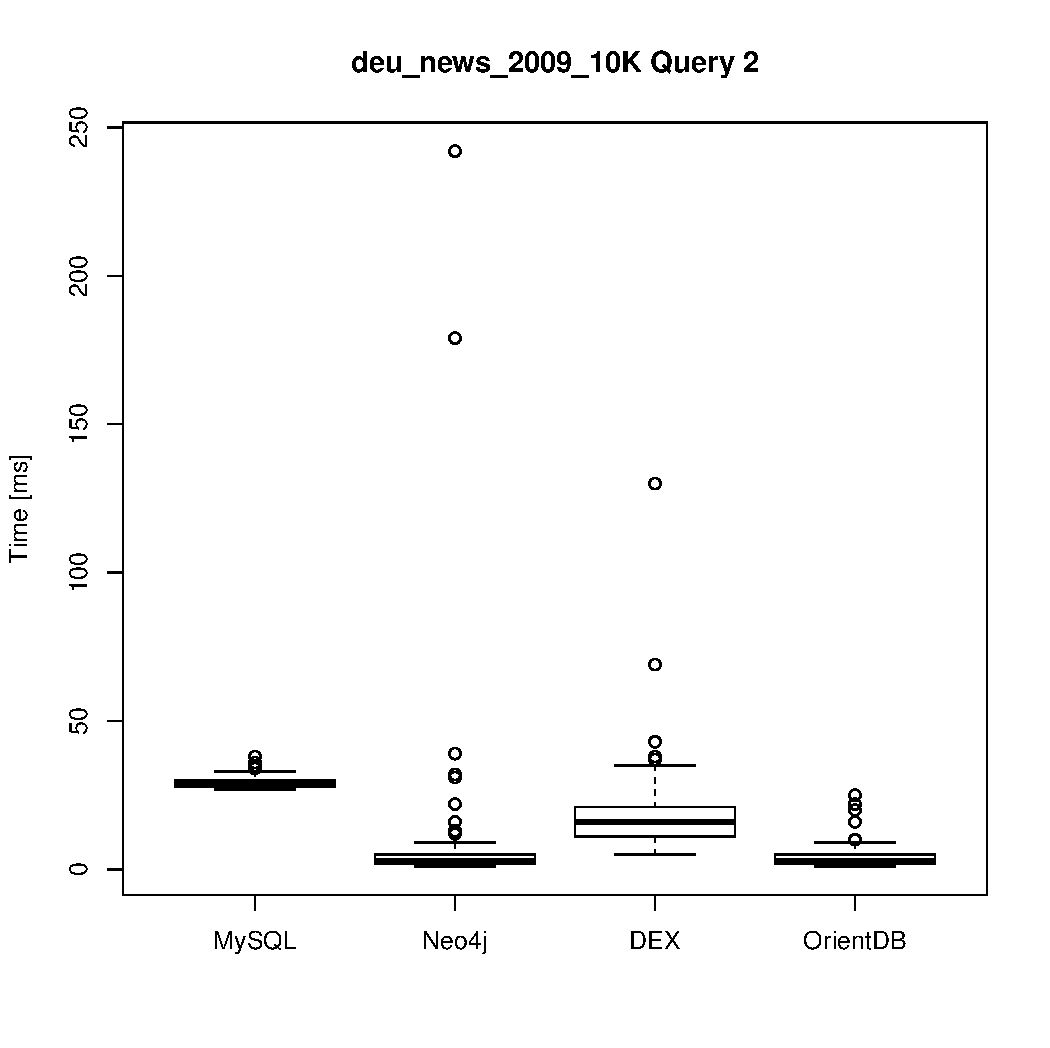
\includegraphics[width=7cm]{../results/cold caches/images/10K_query2_boxplot}
			\label{fig:10K_query2_boxplot}
		\end{minipage}
		\hfill
		\begin{minipage}[hbt]{6.5cm}
			\centering
			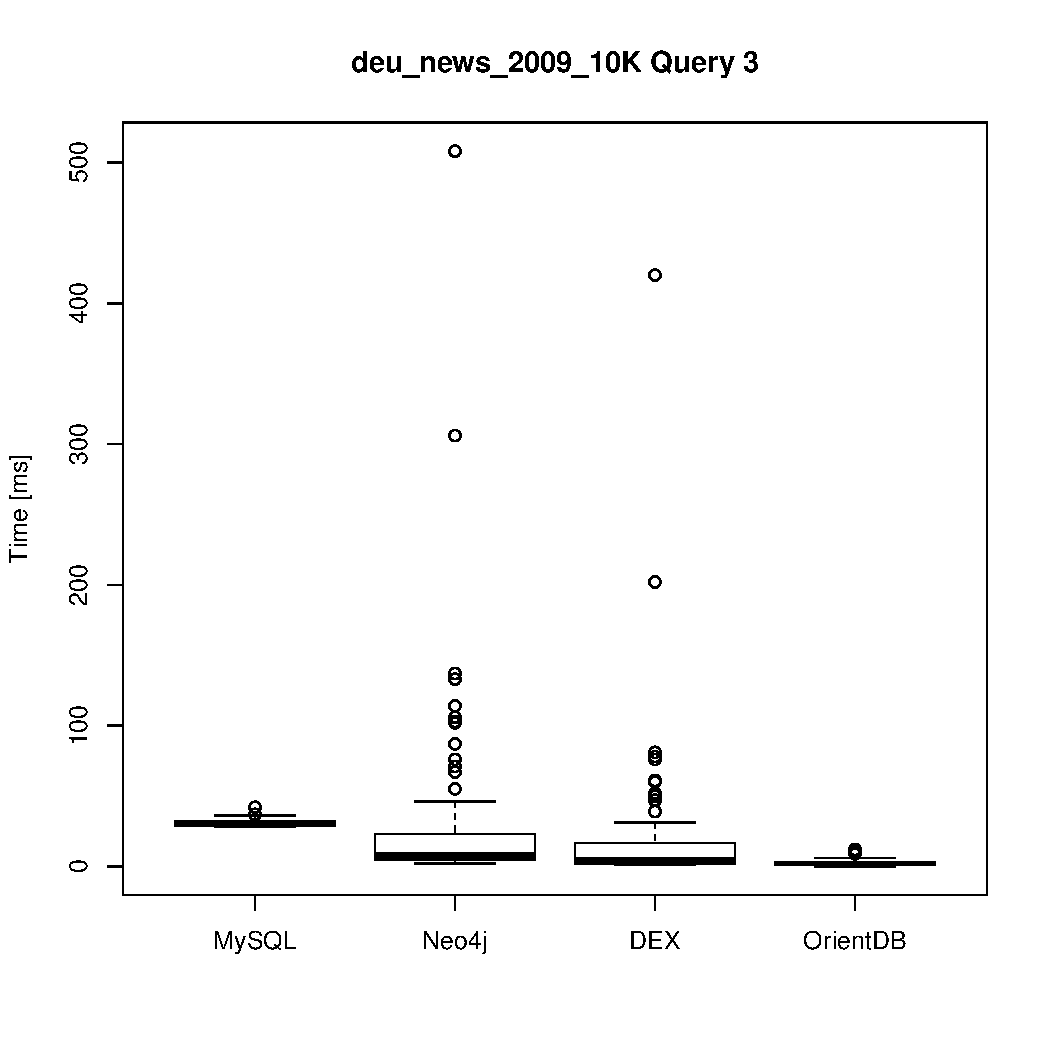
\includegraphics[width=7cm]{../results/cold caches/images/10K_query3_boxplot}
			\label{fig:10K_query3_boxplot}
		\end{minipage}
		
		\begin{minipage}[hbt]{6.5cm}
			\centering
			\includegraphics[width=7cm]{../results/cold caches/images/100K_query1_boxplot}
			\label{fig:100K_query1_boxplot}
		\end{minipage}
		\hfill
		\begin{minipage}[hbt]{6.5cm}
			\centering
			\includegraphics[width=7cm]{../results/cold caches/images/100K_query2_boxplot}
			\label{fig:100K_query2_boxplot}
		\end{minipage}
		\hfill
		\begin{minipage}[hbt]{6.5cm}
			\centering
			\includegraphics[width=7cm]{../results/cold caches/images/100K_query3_boxplot}
			\label{fig:100K_query3_boxplot}
		\end{minipage}
	\end{figure}
\end{landscape} 

\begin{landscape} 
	\newpage
	\thispagestyle{empty}
	
	\begin{figure}[ht]
		\begin{minipage}[hbt]{6.5cm}
			\centering
			\includegraphics[width=7cm]{../results/cold caches/images/1M_query1_boxplot}
			\label{fig:1M_query1_boxplot}
		\end{minipage}
		\hfill
		\begin{minipage}[hbt]{6.5cm}
			\centering
			\includegraphics[width=7cm]{../results/cold caches/images/1M_query2_boxplot}
			\label{fig:1M_query2_boxplot}
		\end{minipage}
		\hfill
		\begin{minipage}[hbt]{6.5cm}
			\centering
			\includegraphics[width=7cm]{../results/cold caches/images/1M_query3_boxplot}
			\label{fig:1M_query3_boxplot}
		\end{minipage}
		
		\begin{minipage}[hbt]{6.5cm}
			\centering
			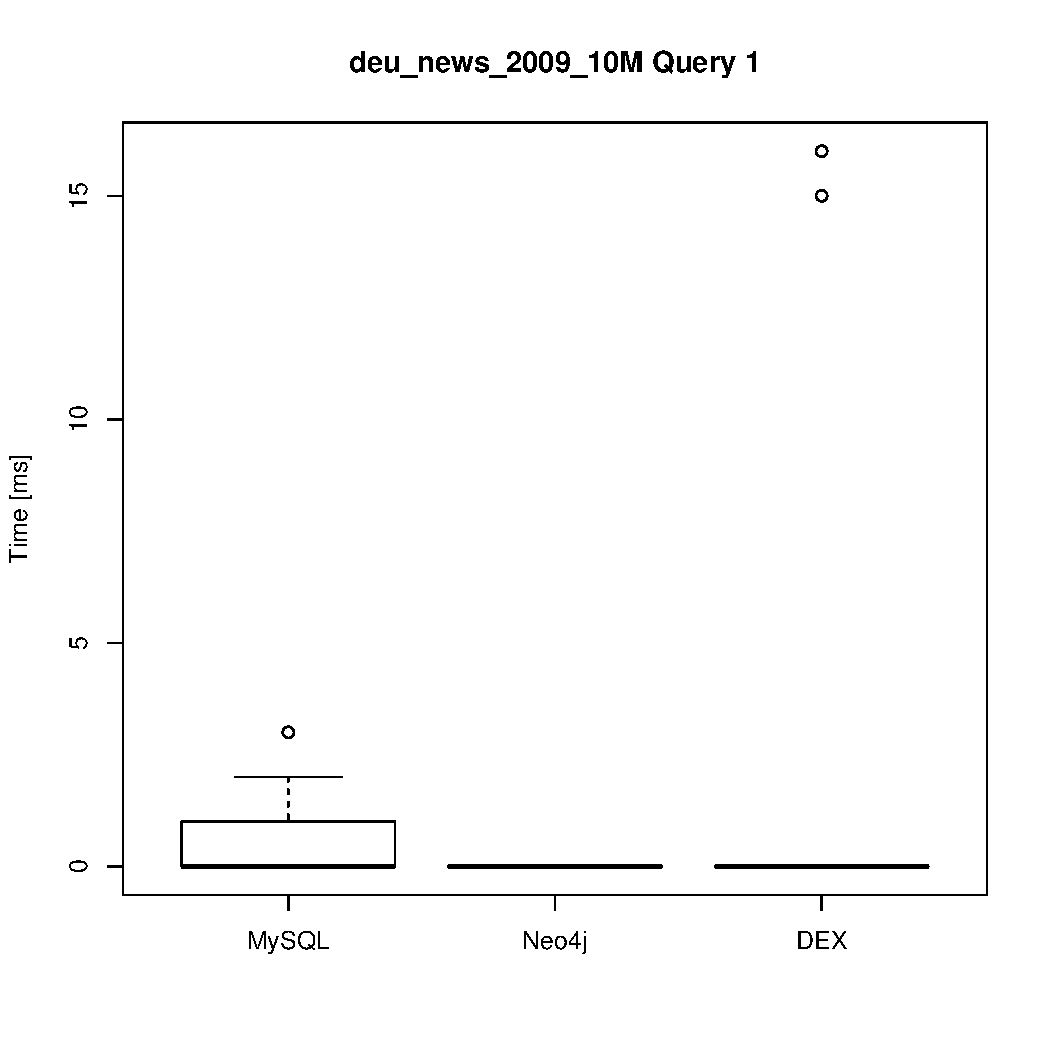
\includegraphics[width=7cm]{../results/cold caches/images/10M_query1_boxplot}
			\label{fig:10M_query1_boxplot}
		\end{minipage}
		\hfill
		\begin{minipage}[hbt]{6.5cm}
			\centering
			\includegraphics[width=7cm]{../results/cold caches/images/10M_query2_boxplot}
			\label{fig:10M_query2_boxplot}
		\end{minipage}
		\hfill
		\begin{minipage}[hbt]{6.5cm}
			\centering
			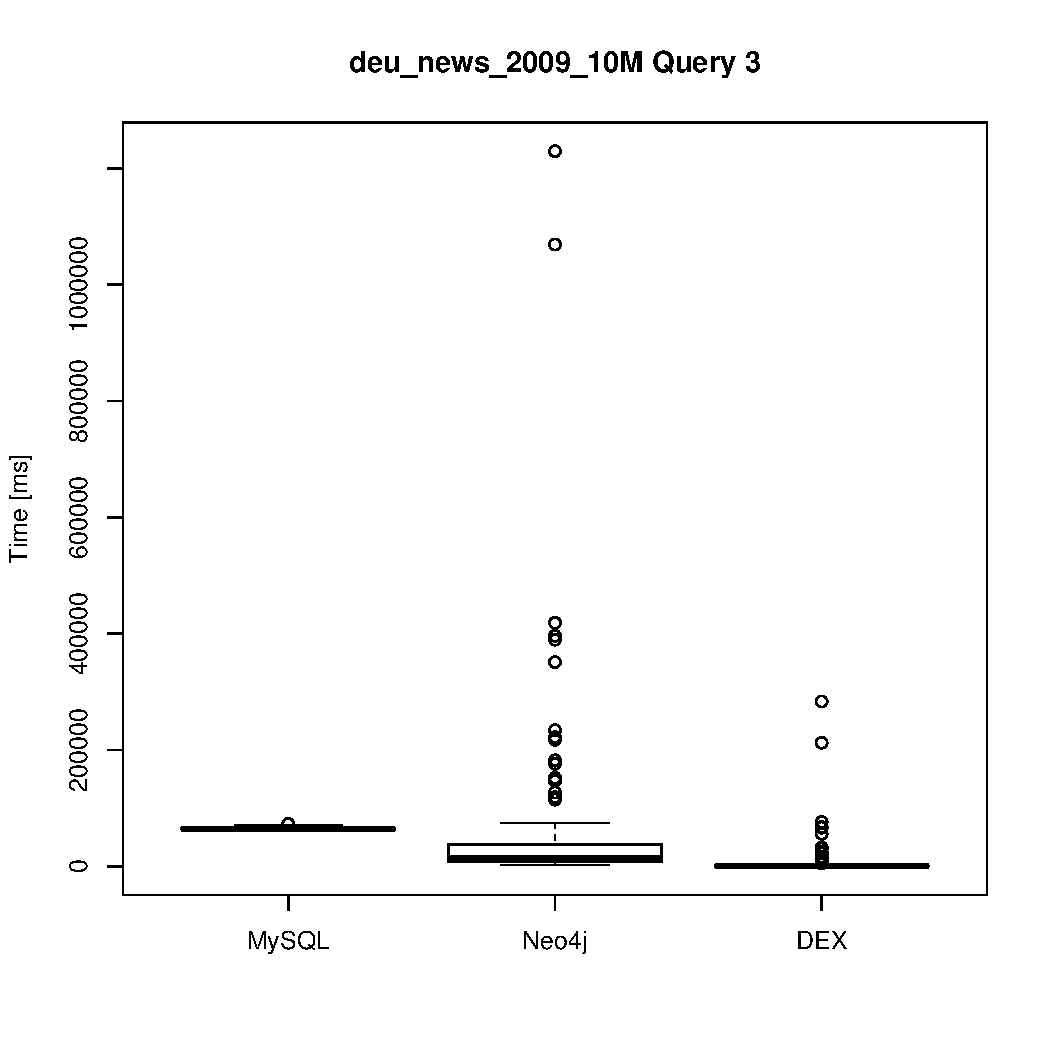
\includegraphics[width=7cm]{../results/cold caches/images/10M_query3_boxplot}
			\label{fig:10M_query3_boxplot}
		\end{minipage}
	\end{figure}
\end{landscape}

\begin{landscape} 
	\newpage
	\thispagestyle{empty}
	
	\begin{figure}[ht]
		\begin{minipage}[hbt]{6.5cm}
			\centering
			\includegraphics[width=7cm]{../results/cold caches/images/10K_query1_perf}
			\label{fig:10K_query1_perf}
		\end{minipage}
		\hfill
		\begin{minipage}[hbt]{6.5cm}
			\centering
			\includegraphics[width=7cm]{../results/cold caches/images/10K_query2_perf}
			\label{fig:10K_query2_perf}
		\end{minipage}
		\hfill
		\begin{minipage}[hbt]{6.5cm}
			\centering
			\includegraphics[width=7cm]{../results/cold caches/images/10K_query3_perf}
			\label{fig:10K_query3_perf}
		\end{minipage}
		
		\begin{minipage}[hbt]{6.5cm}
			\centering
			\includegraphics[width=7cm]{../results/cold caches/images/100K_query1_perf}
			\label{fig:100K_query1_perf}
		\end{minipage}
		\hfill
		\begin{minipage}[hbt]{6.5cm}
			\centering
			\includegraphics[width=7cm]{../results/cold caches/images/100K_query2_perf}
			\label{fig:100K_query2_perf}
		\end{minipage}
		\hfill
		\begin{minipage}[hbt]{6.5cm}
			\centering
			\includegraphics[width=7cm]{../results/cold caches/images/100K_query3_perf}
			\label{fig:100K_query3_perf}
		\end{minipage}
	\end{figure}
\end{landscape} 

\begin{landscape} 
	\newpage
	\thispagestyle{empty}
	
	\begin{figure}[ht]
		\begin{minipage}[hbt]{6.5cm}
			\centering
			\includegraphics[width=7cm]{../results/cold caches/images/1M_query1_perf}
			\label{fig:1M_query1_perf}
		\end{minipage}
		\hfill
		\begin{minipage}[hbt]{6.5cm}
			\centering
			\includegraphics[width=7cm]{../results/cold caches/images/1M_query2_perf}
			\label{fig:1M_query2_perf}
		\end{minipage}
		\hfill
		\begin{minipage}[hbt]{6.5cm}
			\centering
			\includegraphics[width=7cm]{../results/cold caches/images/1M_query3_perf}
			\label{fig:1M_query3_perf}
		\end{minipage}
		
		\begin{minipage}[hbt]{6.5cm}
			\centering
			\includegraphics[width=7cm]{../results/cold caches/images/10M_query1_perf}
			\label{fig:10M_query1_perf}
		\end{minipage}
		\hfill
		\begin{minipage}[hbt]{6.5cm}
			\centering
			\includegraphics[width=7cm]{../results/cold caches/images/10M_query2_perf}
			\label{fig:10M_query2_perf}
		\end{minipage}
		\hfill
		\begin{minipage}[hbt]{6.5cm}
			\centering
			\includegraphics[width=7cm]{../results/cold caches/images/10M_query3_perf}
			\label{fig:10M_query3_perf}
		\end{minipage}
	\end{figure}
\end{landscape}

\begin{landscape} 
	\newpage
	\thispagestyle{empty}
	
	\begin{figure}[ht]
			\centering
			\caption{Klassendiagramm des Benchmarkframeworks inklusive aller Neo4j-Klassen}
			\includegraphics[width=27cm]{pics/class_diagramm_incl_neo4j}
			\label{fig:class_diagramm_neo4j}
	\end{figure}
\end{landscape}

\end{appendix}
\end{document}